\newpage

\onecolumn

\appendix

\section{Skizze zum Versuchsaufbau}
\label{sec:aufbau}
\begin{figure}[htb]
   \centering
   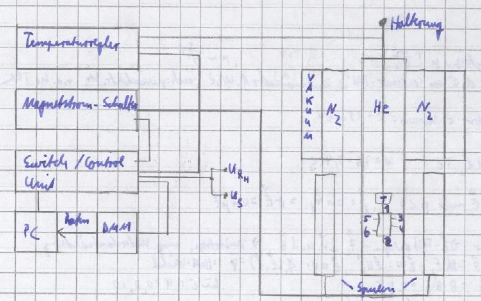
\includegraphics[width=1\columnwidth,keepaspectratio]{aufbau}
   \caption{schematische Skizze des Versuchsaufbaus}
\end{figure}

\section{Messwerte}
\label{sec:messwerte}
OO-Messwerte

auch die ausm laborbuch!!!

\begin{figure}[htb!]
 \centering
 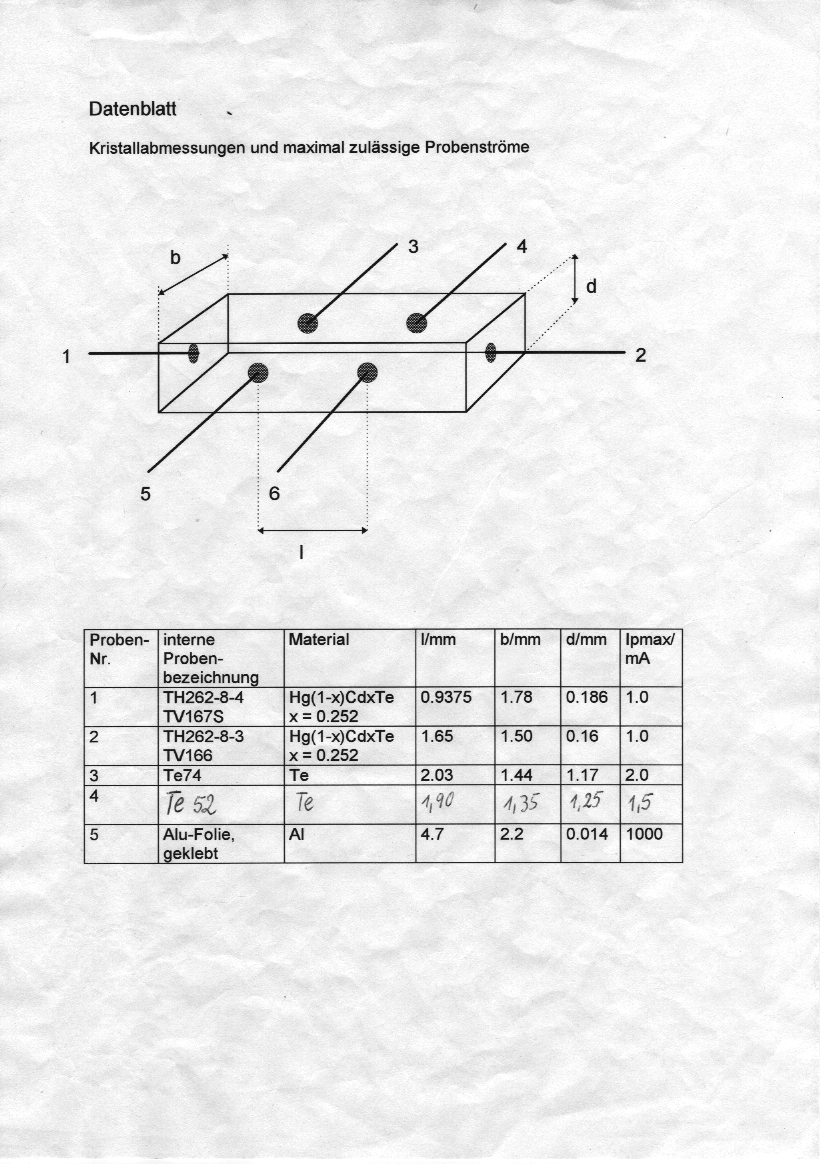
\includegraphics[viewport=40 420 470 700,clip]{../docs/scan_datenblatt}
 % scan_datenblatt.png: 824x1164 pixel, 100dpi, 20.93x29.57 cm, bb=0 0 593 838
 \caption{Abmessungen}
 \label{fig:abmessungen}
\end{figure}



\begin{table}[htb!]
 \centering
 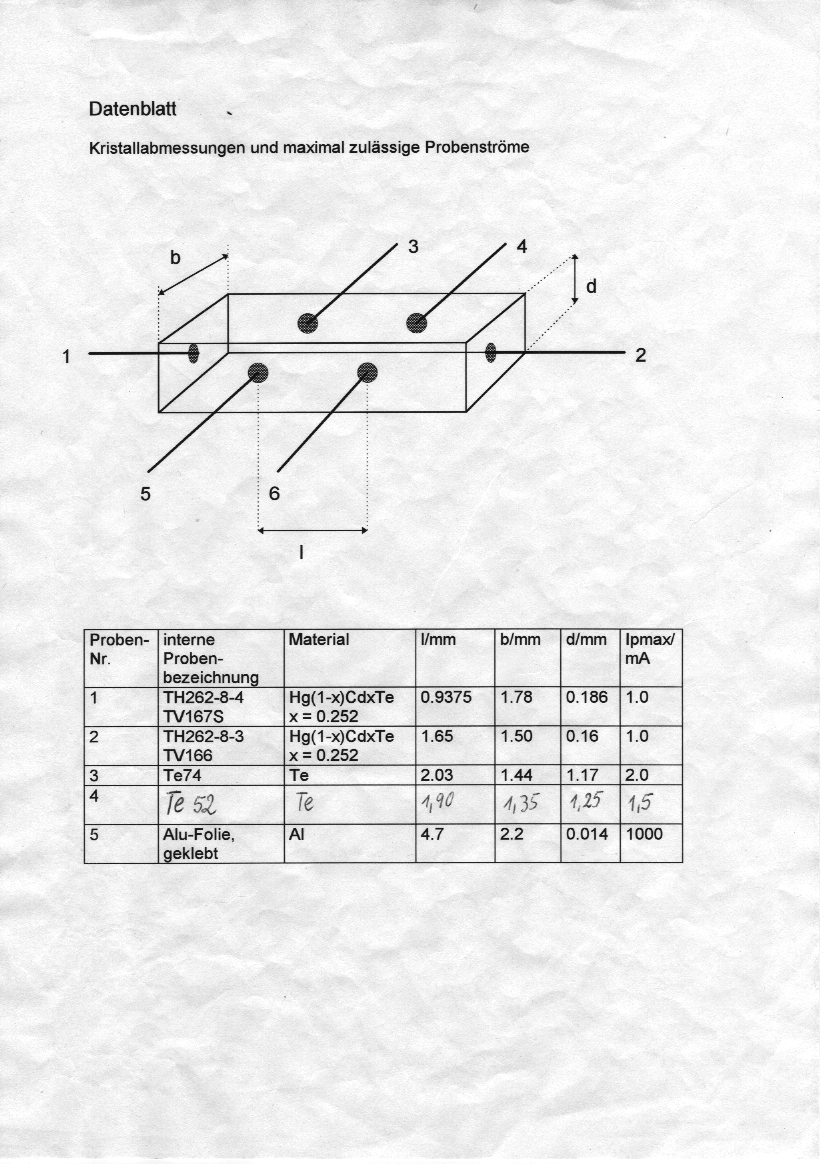
\includegraphics[viewport=55 200 500 390,clip]{../docs/scan_datenblatt}
 % scan_datenblatt.png: 824x1164 pixel, 100dpi, 20.93x29.57 cm, bb=0 0 593 838
 \caption{Daten}
 \label{tab:daten}
\end{table}

\section{Fits}
\label{sec:fits}

\begin{figure}[htbp]
  \subfloat[Abkühl-Phase, mittels ρ]{
    \label{fig:Eg_rho_00}
    \includegraphics[width=0.445\textwidth,keepaspectratio]{../tmp/Eg_rho_00}
  }
  \subfloat[Aufwärm-Phase, mittels ρ]{
    \label{fig:Eg_rho_01}
    \includegraphics[width=0.445\textwidth,keepaspectratio]{../tmp/Eg_rho_01}
  }
  \newline
  \subfloat[Abkühl-Phase, mittels $R_H$]{
    \label{fig:Eg_R_H_00}
    \includegraphics[width=0.445\textwidth,keepaspectratio]{../tmp/Eg_R_H_00}
  }
  \subfloat[Aufwärm-Phase, mittels $R_H$]{
    \label{fig:Eg_R_H_01}
    \includegraphics[width=0.445\textwidth,keepaspectratio]{../tmp/Eg_R_H_01}
  }
  \caption{Lineare Regression zur Bestimmung der Bandlücke $E_g$}
  \label{fig:ohne_hintergrund}
\end{figure}